\documentclass{ntuabeamer}

\usepackage[utf8]{inputenc}
\usepackage{amsmath}
\usepackage{amssymb}
\usepackage{graphicx}
\usepackage{tikz}
\usetikzlibrary{arrows.meta,calc,positioning}

\title{Convolutional Neural Networks}
\author{}
\date{}

\definecolor{courseblue}{HTML}{3F7CAC}
\definecolor{courseorange}{HTML}{D97706}
\definecolor{coursegreen}{HTML}{27864A}
\definecolor{coursegray}{HTML}{667085}
\definecolor{coursepurple}{HTML}{7656A3}
\definecolor{coursered}{HTML}{B5473C}
\definecolor{courselightblue}{HTML}{DCE9F5}
\definecolor{courselightorange}{HTML}{F9E4C8}

\tikzset{
  flow/.style={-{Latex[length=3mm]},very thick,courseblue},
  box/.style={draw,rounded corners,very thick,align=center,minimum height=0.9cm},
  unit/.style={circle,draw,very thick,minimum size=0.42cm,inner sep=0pt},
  cell/.style={draw,minimum size=0.58cm,inner sep=0pt}
}

\begin{document}

\begin{frame}[plain]
  \makepresentationtitle
\end{frame}

\begin{frame}{Dense Connectivity Ignores Spatial Locality}
  \centering
  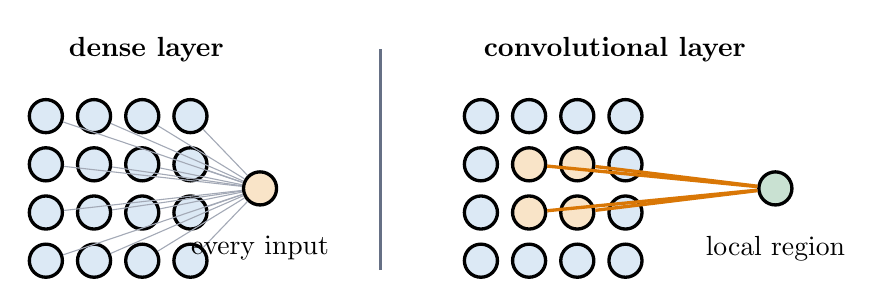
\begin{tikzpicture}[scale=0.85]
    \node[font=\bfseries] at (-3.5,3.0) {dense layer};
    \foreach \i in {0,...,3}{
      \foreach \j in {0,...,3}{
        \node[unit,fill=courselightblue] (d\i\j) at (-5+0.72*\i,2.0-0.72*\j) {};
      }
    }
    \node[unit,fill=courselightorange] (do) at (-1.8,0.92) {};
    \foreach \i in {0,...,3}{
      \foreach \j in {0,...,3}{\draw[coursegray!60] (d\i\j) -- (do);}
    }
    \node[below=0.25cm of do] {every input};

    \draw[coursegray,very thick] (0,-0.3) -- (0,3.0);

    \node[font=\bfseries] at (3.5,3.0) {convolutional layer};
    \foreach \i in {0,...,3}{
      \foreach \j in {0,...,3}{
        \pgfmathtruncatemacro{\inside}{(\i>0 && \i<3 && \j>0 && \j<3)}
        \ifnum\inside=1
          \node[unit,fill=courselightorange] (c\i\j) at (1.5+0.72*\i,2.0-0.72*\j) {};
        \else
          \node[unit,fill=courselightblue] (c\i\j) at (1.5+0.72*\i,2.0-0.72*\j) {};
        \fi
      }
    }
    \node[unit,fill=coursegreen!25] (co) at (5.9,0.92) {};
    \foreach \i in {1,2}{
      \foreach \j in {1,2}{\draw[courseorange,very thick] (c\i\j) -- (co);}
    }
    \node[below=0.25cm of co] {local region};
  \end{tikzpicture}
\end{frame}

\begin{frame}{A Kernel Sees One Local Receptive Field}
  \centering
  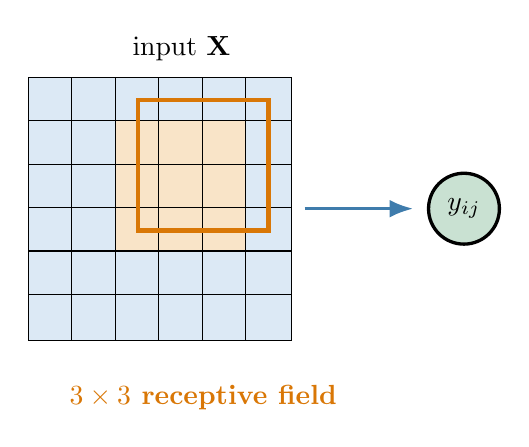
\begin{tikzpicture}[scale=0.92]
    \foreach \r in {0,...,5}{
      \foreach \c in {0,...,5}{
        \pgfmathtruncatemacro{\inside}{(\r>0 && \r<4 && \c>1 && \c<5)}
        \ifnum\inside=1
          \node[cell,fill=courselightorange] at (0.6*\c,-0.6*\r) {};
        \else
          \node[cell,fill=courselightblue] at (0.6*\c,-0.6*\r) {};
        \fi
      }
    }
    \draw[courseorange,ultra thick] (1.2,0) rectangle (3.0,-1.8);
    \node[above] at (1.8,0.4) {input $\mathbf{X}$};
    \node[below,courseorange,font=\bfseries] at (2.1,-3.8) {$3\times3$ receptive field};
    \draw[flow] (3.5,-1.5) -- (5.0,-1.5);
    \node[unit,fill=coursegreen!25,minimum size=0.9cm] at (5.7,-1.5) {$y_{ij}$};
  \end{tikzpicture}
\end{frame}

\begin{frame}{One Output Is a Local Weighted Sum}
  \centering
  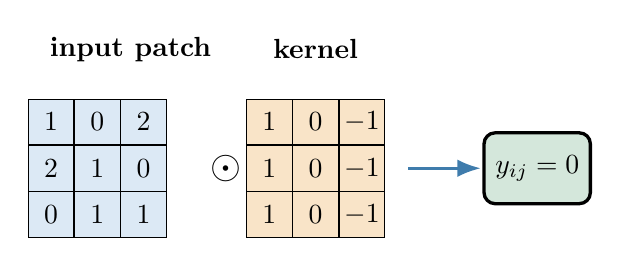
\begin{tikzpicture}[scale=0.84]
    \node[font=\bfseries] at (1.2,1.1) {input patch};
    \foreach \r/\row in {0/{1,0,2},1/{2,1,0},2/{0,1,1}}{
      \foreach \value [count=\c from 0] in \row{
        \node[cell,fill=courselightblue] at (0.7*\c,-0.7*\r) {$\value$};
      }
    }
    \node[font=\bfseries] at (4.0,1.1) {kernel};
    \foreach \r/\row in {0/{1,0,-1},1/{1,0,-1},2/{1,0,-1}}{
      \foreach \value [count=\c from 0] in \row{
        \node[cell,fill=courselightorange] at (3.3+0.7*\c,-0.7*\r) {$\value$};
      }
    }
    \node[font=\Large] at (2.65,-0.7) {$\odot$};
    \draw[flow] (5.4,-0.7) -- (6.5,-0.7);
    \node[box,fill=coursegreen!20,minimum width=1.35cm] at (7.35,-0.7) {$y_{ij}=0$};
  \end{tikzpicture}
  \vspace{0.5cm}
  \[
    y_{ij}=b+\sum_{u=0}^{K_h-1}\sum_{v=0}^{K_w-1}
    K_{uv}\,X_{i+u,j+v}
  \]
  \begin{itemize}
    \item Libraries usually compute cross-correlation and call it convolution.
  \end{itemize}
\end{frame}

\begin{frame}{Sliding the Kernel Builds a Feature Map}
  \centering
  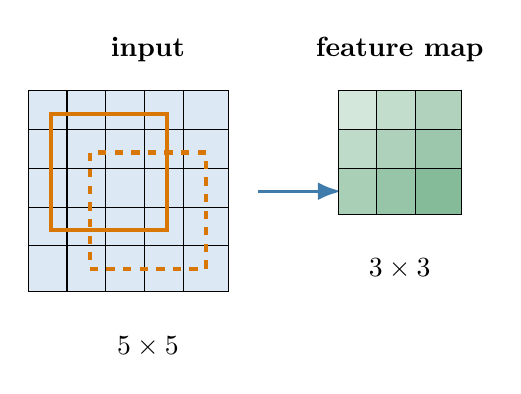
\begin{tikzpicture}[scale=0.82]
    \node[font=\bfseries] at (1.5,1.0) {input};
    \foreach \r in {0,...,4}{
      \foreach \c in {0,...,4}{\node[cell,fill=courselightblue] at (0.6*\c,-0.6*\r) {};}
    }
    \draw[courseorange,ultra thick] (0,0) rectangle (1.8,-1.8);
    \draw[courseorange,ultra thick,dashed] (0.6,-0.6) rectangle (2.4,-2.4);
    \draw[flow] (3.2,-1.2) -- (4.5,-1.2);
    \node[font=\bfseries] at (5.4,1.0) {feature map};
    \foreach \r in {0,...,2}{
      \foreach \c in {0,...,2}{
        \pgfmathtruncatemacro{\shade}{20+10*\r+8*\c}
        \node[cell,fill=coursegreen!\shade] at (4.8+0.6*\c,-0.6*\r) {};
      }
    }
    \node[below] at (1.5,-3.3) {$5\times5$};
    \node[below] at (5.4,-2.1) {$3\times3$};
  \end{tikzpicture}
\end{frame}

\begin{frame}{Channels Separate Different Learned Features}
  \centering
  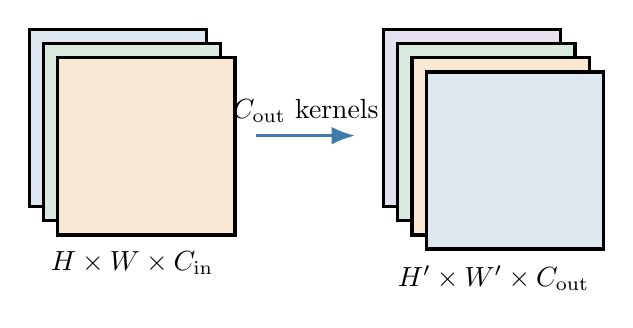
\begin{tikzpicture}[scale=0.9]
    \foreach \k/\color in {0/courseblue,1/coursegreen,2/courseorange}{
      \draw[very thick,fill=\color!18] (0.2*\k,-0.2*\k) rectangle ++(2.5,-2.5);
    }
    \node[below] at (1.45,-3.0) {$H\times W\times C_{\mathrm{in}}$};
    \draw[flow] (3.2,-1.5) -- (4.6,-1.5);
    \node[above] at (3.9,-1.45) {$C_{\mathrm{out}}$ kernels};
    \foreach \k/\color in {0/coursepurple,1/coursegreen,2/courseorange,3/courseblue}{
      \draw[very thick,fill=\color!18] (5.0+0.2*\k,-0.2*\k) rectangle ++(2.5,-2.5);
    }
    \node[below] at (6.55,-3.2) {$H'\times W'\times C_{\mathrm{out}}$};
  \end{tikzpicture}
  \vspace{0.4cm}
  \[
    K\in\mathbb{R}^{K_h\times K_w\times C_{\mathrm{in}}\times C_{\mathrm{out}}}
  \]
\end{frame}

\begin{frame}{The Same Kernel Is Shared Across Space}
  \centering
  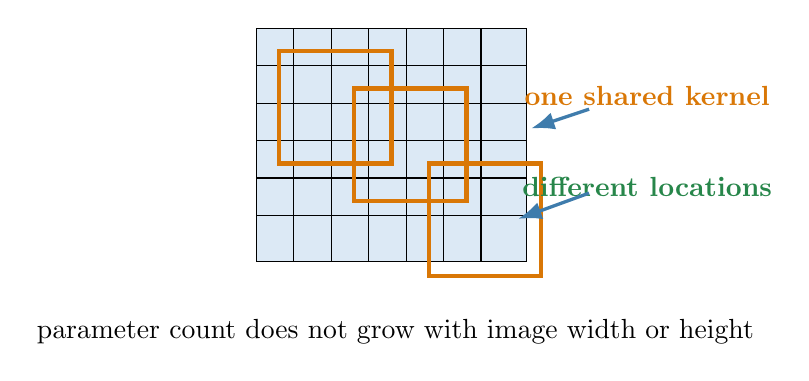
\begin{tikzpicture}[scale=0.82]
    \foreach \r in {0,...,5}{
      \foreach \c in {0,...,6}{\node[cell,fill=courselightblue] at (0.58*\c,-0.58*\r) {};}
    }
    \foreach \x/\y in {0/0,1.16/-0.58,2.32/-1.74}{
      \draw[courseorange,ultra thick] (\x,\y) rectangle ++(1.74,-1.74);
    }
    \node[courseorange,font=\bfseries] at (5.7,-0.7) {one shared kernel};
    \draw[flow] (4.8,-0.9) -- (3.9,-1.2);
    \node[coursegreen,font=\bfseries] at (5.7,-2.1) {different locations};
    \draw[flow] (4.8,-2.2) -- (3.7,-2.6);
    \node[below] at (1.8,-4.0) {parameter count does not grow with image width or height};
  \end{tikzpicture}
\end{frame}

\begin{frame}{Shared Kernels Produce Translation Equivariance}
  Ignoring boundaries and sampling, shifting the input shifts the feature map:
  \[
    \operatorname{Conv}_{K}(T_u\mathbf X)
    =T_u\operatorname{Conv}_{K}(\mathbf X).
  \]
  \begin{itemize}
    \item The same local rule is evaluated at every spatial location.
    \item A feature does not need to be relearned separately at every coordinate.
    \item Global pooling may turn an equivariant representation into an invariant prediction.
  \end{itemize}
  The geometric-deep-learning lecture proves this identity formally.
\end{frame}

\begin{frame}{Receptive Fields Grow across Layers}
  Let $r_\ell$ be receptive-field size and $j_\ell$ the input spacing between
  neighboring layer-$\ell$ features. Starting with $r_0=j_0=1$,
  \[
    j_\ell=j_{\ell-1}S_\ell,
    \qquad
    r_\ell=r_{\ell-1}+(K_\ell-1)D_\ell j_{\ell-1}.
  \]
  Three stride-one $3\times3$ layers have receptive fields
  \[
    3\times3\ \longrightarrow\ 5\times5\ \longrightarrow\ 7\times7.
  \]
  Depth combines local operations into progressively wider context.
\end{frame}

\begin{frame}{Stride Controls How Far the Kernel Moves}
  \centering
  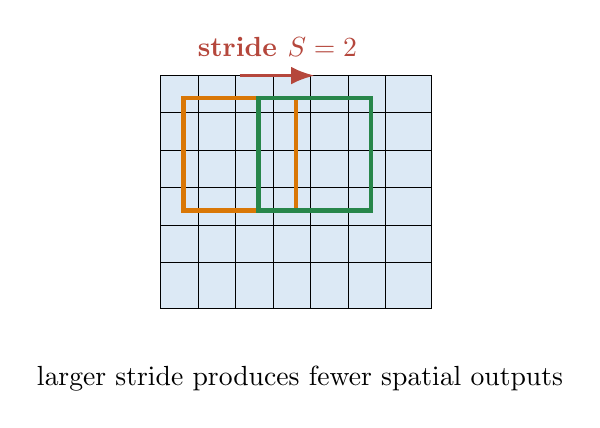
\begin{tikzpicture}[scale=0.82]
    \foreach \r in {0,...,5}{
      \foreach \c in {0,...,6}{\node[cell,fill=courselightblue] at (0.58*\c,-0.58*\r) {};}
    }
    \draw[courseorange,ultra thick] (0,0) rectangle ++(1.74,-1.74);
    \draw[coursegreen,ultra thick] (1.16,0) rectangle ++(1.74,-1.74);
    \draw[-{Latex[length=3mm]},very thick,coursered] (0.87,0.35) -- (2.03,0.35);
    \node[above,coursered,font=\bfseries] at (1.45,0.5) {stride $S=2$};
    \node[below] at (1.8,-4.0) {larger stride produces fewer spatial outputs};
  \end{tikzpicture}
\end{frame}

\begin{frame}{Dilation Expands Support without More Kernel Weights}
  In one spatial dimension,
  \[
    y_i=\sum_{u=0}^{K-1}k_u\,x_{i+D u}.
  \]
  The effective kernel size is
  \[
    K_{\mathrm{eff}}=D(K-1)+1.
  \]
  A $3$-tap kernel with dilation $D=2$ spans $5$ input positions but still learns only three weights per channel pair.
\end{frame}

\begin{frame}{Padding Preserves Information Near Boundaries}
  \centering
  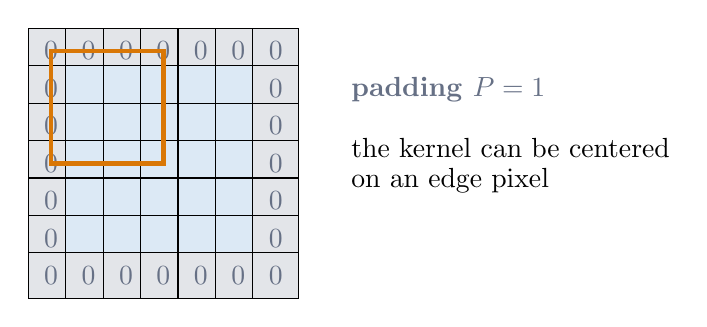
\begin{tikzpicture}[scale=0.82]
    \foreach \r in {0,...,6}{
      \foreach \c in {0,...,6}{
        \pgfmathtruncatemacro{\border}{(\r==0 || \r==6 || \c==0 || \c==6)}
        \ifnum\border=1
          \node[cell,fill=coursegray!18,text=coursegray] at (0.58*\c,-0.58*\r) {$0$};
        \else
          \node[cell,fill=courselightblue] at (0.58*\c,-0.58*\r) {};
        \fi
      }
    }
    \draw[courseorange,ultra thick] (0,0) rectangle ++(1.74,-1.74);
    \node[right,coursegray,font=\bfseries] at (4.5,-0.6) {padding $P=1$};
    \node[right] at (4.5,-1.5) {the kernel can be centered};
    \node[right] at (4.5,-2.0) {on an edge pixel};
  \end{tikzpicture}
\end{frame}

\begin{frame}{Kernel, Dilation, Padding, and Stride Set Output Size}
  For each spatial dimension:
  \[
    \boxed{
      O=\left\lfloor
      \frac{I+2P-D(K-1)-1}{S}
      \right\rfloor+1
    }
  \]
  \begin{itemize}
    \item $I$: input size.
    \item $K$: kernel size.
    \item $D$: dilation.
    \item $P$: padding on each side.
    \item $S$: stride.
  \end{itemize}
  \[
    I=5,\quad K=3,\quad D=1,\quad P=1,\quad S=1
    \quad\Longrightarrow\quad O=5
  \]
\end{frame}

\begin{frame}{Padding and Stride Limit Exact Equivariance}
  \begin{itemize}
    \item Zero padding treats the image boundary differently from its interior.
    \item Stride keeps one sampling phase; a one-pixel shift can change which values survive.
    \item Downsampling without adequate low-pass filtering can alias high frequencies.
  \end{itemize}
  Translation equivariance is exact for the ideal operator, not automatically for every finite CNN implementation.
\end{frame}

\begin{frame}{Pooling Is One Optional Downsampling Choice}
  \centering
  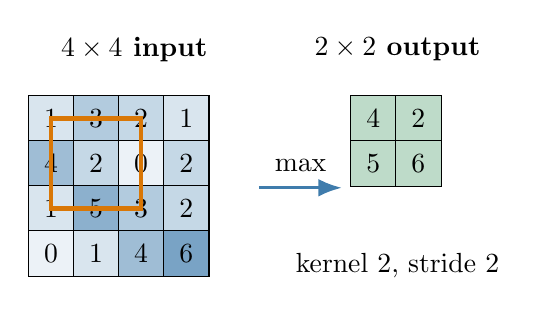
\begin{tikzpicture}[scale=0.88]
    \node[font=\bfseries] at (1.2,1.0) {$4\times4$ input};
    \foreach \r/\row in {0/{1,3,2,1},1/{4,2,0,2},2/{1,5,3,2},3/{0,1,4,6}}{
      \foreach \value [count=\c from 0] in \row{
        \pgfmathtruncatemacro{\shade}{10+10*\value}
        \node[cell,fill=courseblue!\shade] at (0.65*\c,-0.65*\r) {$\value$};
      }
    }
    \draw[courseorange,ultra thick] (0,0) rectangle (1.3,-1.3);
    \draw[flow] (3.0,-1.0) -- (4.2,-1.0);
    \node[above] at (3.6,-0.9) {max};
    \node[font=\bfseries] at (5.0,1.0) {$2\times2$ output};
    \foreach \r/\row in {0/{4,2},1/{5,6}}{
      \foreach \value [count=\c from 0] in \row{
        \node[cell,fill=coursegreen!30] at (4.65+0.65*\c,-0.65*\r) {$\value$};
      }
    }
    \node[below] at (5.0,-1.8) {kernel $2$, stride $2$};
  \end{tikzpicture}
  \vspace{0.45cm}
  \begin{itemize}
    \item A strided convolution can also downsample.
  \end{itemize}
\end{frame}

\begin{frame}{Parameter Sharing Makes Convolution Efficient}
  \[
    \underbrace{K_hK_wC_{\mathrm{in}}C_{\mathrm{out}}
    +C_{\mathrm{out}}}_{\text{convolution parameters}}
  \]
  \begin{itemize}
    \item One bias is commonly learned per output channel.
    \item The count is independent of $H$ and $W$.
  \end{itemize}
  \vspace{0.35cm}
  \[
    K_h=K_w=3,\quad C_{\mathrm{in}}=3,\quad C_{\mathrm{out}}=16
  \]
  \[
    3\cdot3\cdot3\cdot16+16=448
  \]
\end{frame}

\begin{frame}{A CNN Builds Features Hierarchically}
  \centering
  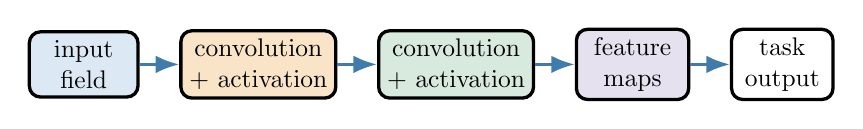
\begin{tikzpicture}[node distance=0.55cm,scale=0.92,transform shape]
    \node[box,fill=courselightblue,minimum width=1.5cm] (input) {input\\field};
    \node[box,fill=courselightorange,minimum width=1.8cm,right=of input] (conv1) {convolution\\$+$ activation};
    \node[box,fill=coursegreen!18,minimum width=1.8cm,right=of conv1] (conv2) {convolution\\$+$ activation};
    \node[box,fill=coursepurple!18,minimum width=1.55cm,right=of conv2] (features) {feature\\maps};
    \node[box,fill=white,minimum width=1.4cm,right=of features] (output) {task\\output};
    \draw[flow] (input) -- (conv1);
    \draw[flow] (conv1) -- (conv2);
    \draw[flow] (conv2) -- (features);
    \draw[flow] (features) -- (output);
  \end{tikzpicture}
  \vspace{0.65cm}
  \begin{itemize}
    \item Pooling is optional.
    \item A fully connected head is optional.
  \end{itemize}
\end{frame}

\begin{frame}{Classification Produces One Prediction per Input}
  \centering
  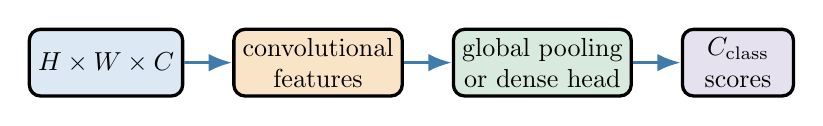
\begin{tikzpicture}[node distance=0.65cm,scale=0.94,transform shape]
    \node[box,fill=courselightblue,minimum width=1.7cm] (field) {$H\times W\times C$};
    \node[box,fill=courselightorange,minimum width=2.0cm,right=of field] (cnn) {convolutional\\features};
    \node[box,fill=coursegreen!18,minimum width=1.9cm,right=of cnn] (pool) {global pooling\\or dense head};
    \node[box,fill=coursepurple!18,minimum width=1.5cm,right=of pool] (class) {$C_{\mathrm{class}}$\\scores};
    \draw[flow] (field) -- (cnn);
    \draw[flow] (cnn) -- (pool);
    \draw[flow] (pool) -- (class);
  \end{tikzpicture}
\end{frame}

\begin{frame}{Spatial Tasks Produce One Prediction per Location}
  \centering
  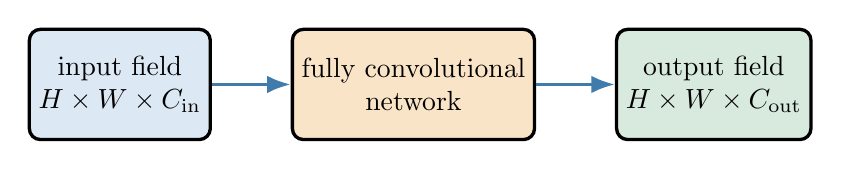
\begin{tikzpicture}[node distance=1.0cm]
    \node[box,fill=courselightblue,minimum width=2.0cm,minimum height=1.4cm] (input) {input field\\$H\times W\times C_{\mathrm{in}}$};
    \node[box,fill=courselightorange,minimum width=2.1cm,minimum height=1.4cm,right=of input] (cnn) {fully convolutional\\network};
    \node[box,fill=coursegreen!18,minimum width=2.2cm,minimum height=1.4cm,right=of cnn] (output) {output field\\$H\times W\times C_{\mathrm{out}}$};
    \draw[flow] (input) -- (cnn);
    \draw[flow] (cnn) -- (output);
  \end{tikzpicture}
  \vspace{0.7cm}
  \begin{itemize}
    \item Examples include segmentation and surrogate field prediction.
  \end{itemize}
\end{frame}

\begin{frame}{Encoder--Decoder Networks Recover Spatial Resolution}
  \centering
  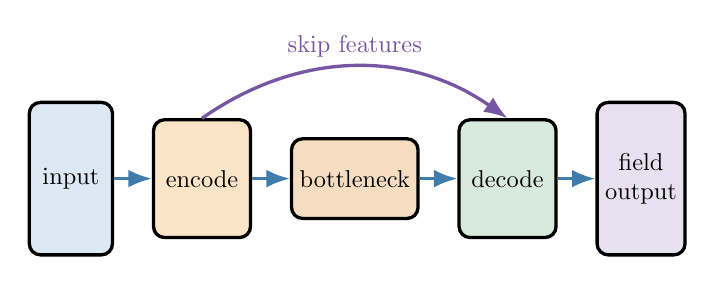
\begin{tikzpicture}[node distance=0.55cm,scale=0.88,transform shape]
    \node[box,fill=courselightblue,minimum width=1.2cm,minimum height=2.2cm] (x) {input};
    \node[box,fill=courselightorange,minimum width=1.4cm,minimum height=1.7cm,right=of x] (e1) {encode};
    \node[box,fill=courseorange!25,minimum width=1.4cm,minimum height=1.15cm,right=of e1] (e2) {bottleneck};
    \node[box,fill=coursegreen!18,minimum width=1.4cm,minimum height=1.7cm,right=of e2] (d1) {decode};
    \node[box,fill=coursepurple!18,minimum width=1.2cm,minimum height=2.2cm,right=of d1] (y) {field\\output};
    \draw[flow] (x)--(e1); \draw[flow] (e1)--(e2); \draw[flow] (e2)--(d1); \draw[flow] (d1)--(y);
    \draw[-{Latex[length=3mm]},very thick,coursepurple,bend left=35]
      (e1.north) to node[above]{skip features} (d1.north);
  \end{tikzpicture}

  Skip connections restore fine spatial information that a compressed bottleneck may lose.
\end{frame}

\begin{frame}{CNNs Also Process Scientific Grids and Fields}
  \begin{itemize}
    \item Images: classification, detection, and segmentation.
    \item Time--frequency maps: audio and vibration diagnostics.
    \item Structured meshes or voxels: stress, flow, temperature, and medical volumes.
  \end{itemize}
  The grid spacing, boundary conditions, channels, and target transformation determine whether the convolutional prior is appropriate.
\end{frame}

\begin{frame}{Local Shared Operators Have Limits}
  \begin{itemize}
    \item Long-range interaction may require many layers or explicit global mechanisms.
    \item Downsampling can discard phase and fine-scale information.
    \item Boundaries and irregular geometry violate the ideal translation model.
    \item Memory and computation grow with spatial resolution and channel count.
  \end{itemize}
  Use a CNN because locality and translation structure match the task, not merely because the input can be stored as an array.
\end{frame}

\begin{frame}{CNNs Encode a Spatial Prior}
  \begin{itemize}
    \item Local receptive fields exploit nearby structure.
    \item Shared kernels detect a feature across locations.
    \item Channels represent different learned features.
    \item Stride and padding control spatial resolution.
    \item Pooling and dense heads are design choices.
    \item CNNs support classification and spatial outputs.
  \end{itemize}
\end{frame}

\end{document}
